\section{Thiết kế UI và UX}
Thiết kế UI và UX của DigitalBookLLM không chỉ phục vụ mục tiêu thẩm mỹ mà còn là một phần của lời giải kỹ thuật cho bài toán đứt gãy ngữ cảnh khi làm việc với tài liệu dài. Toàn bộ giao diện được xây dựng theo hướng ưu tiên không gian đọc, khả năng tương tác trực tiếp với tài liệu và phản hồi theo thời gian thực.

\subsection{Nguyên tắc thiết kế cốt lõi}
Giao diện của hệ thống được xây dựng theo triết lý \textit{knowledge-centric design}, tức là ưu tiên tối đa cho không gian đọc, suy luận và tương tác với tài liệu.

\begin{itemize}
    \item \textbf{Tính nhất quán về ngữ cảnh.} Luôn duy trì sự hiện diện song song của tài liệu gốc và cửa sổ hội thoại.
    \item \textbf{Phản hồi tức thì.} Sử dụng cơ chế streaming để hiển thị câu trả lời ngay trong khi mô hình đang suy luận.
    \item \textbf{Tương tác hai chiều.} Không chỉ người dùng đặt câu hỏi cho AI, mà AI còn có khả năng điều hướng người dùng quay trở lại đúng vị trí trong tài liệu thông qua hệ thống trích dẫn.
\end{itemize}

\subsection{Đặc tả các màn hình chức năng chính}
\subsubsection{Màn hình thư viện tri thức}
Đây là nơi người dùng quản lý các tài liệu đã nạp vào hệ thống. UI cần thể hiện được tính trực quan và trạng thái xử lý của từng tệp.

\begin{figure}[H]
    \centering
    \caption{Giao diện thư viện tri thức của hệ thống}
    \label{fig:ui-library}
    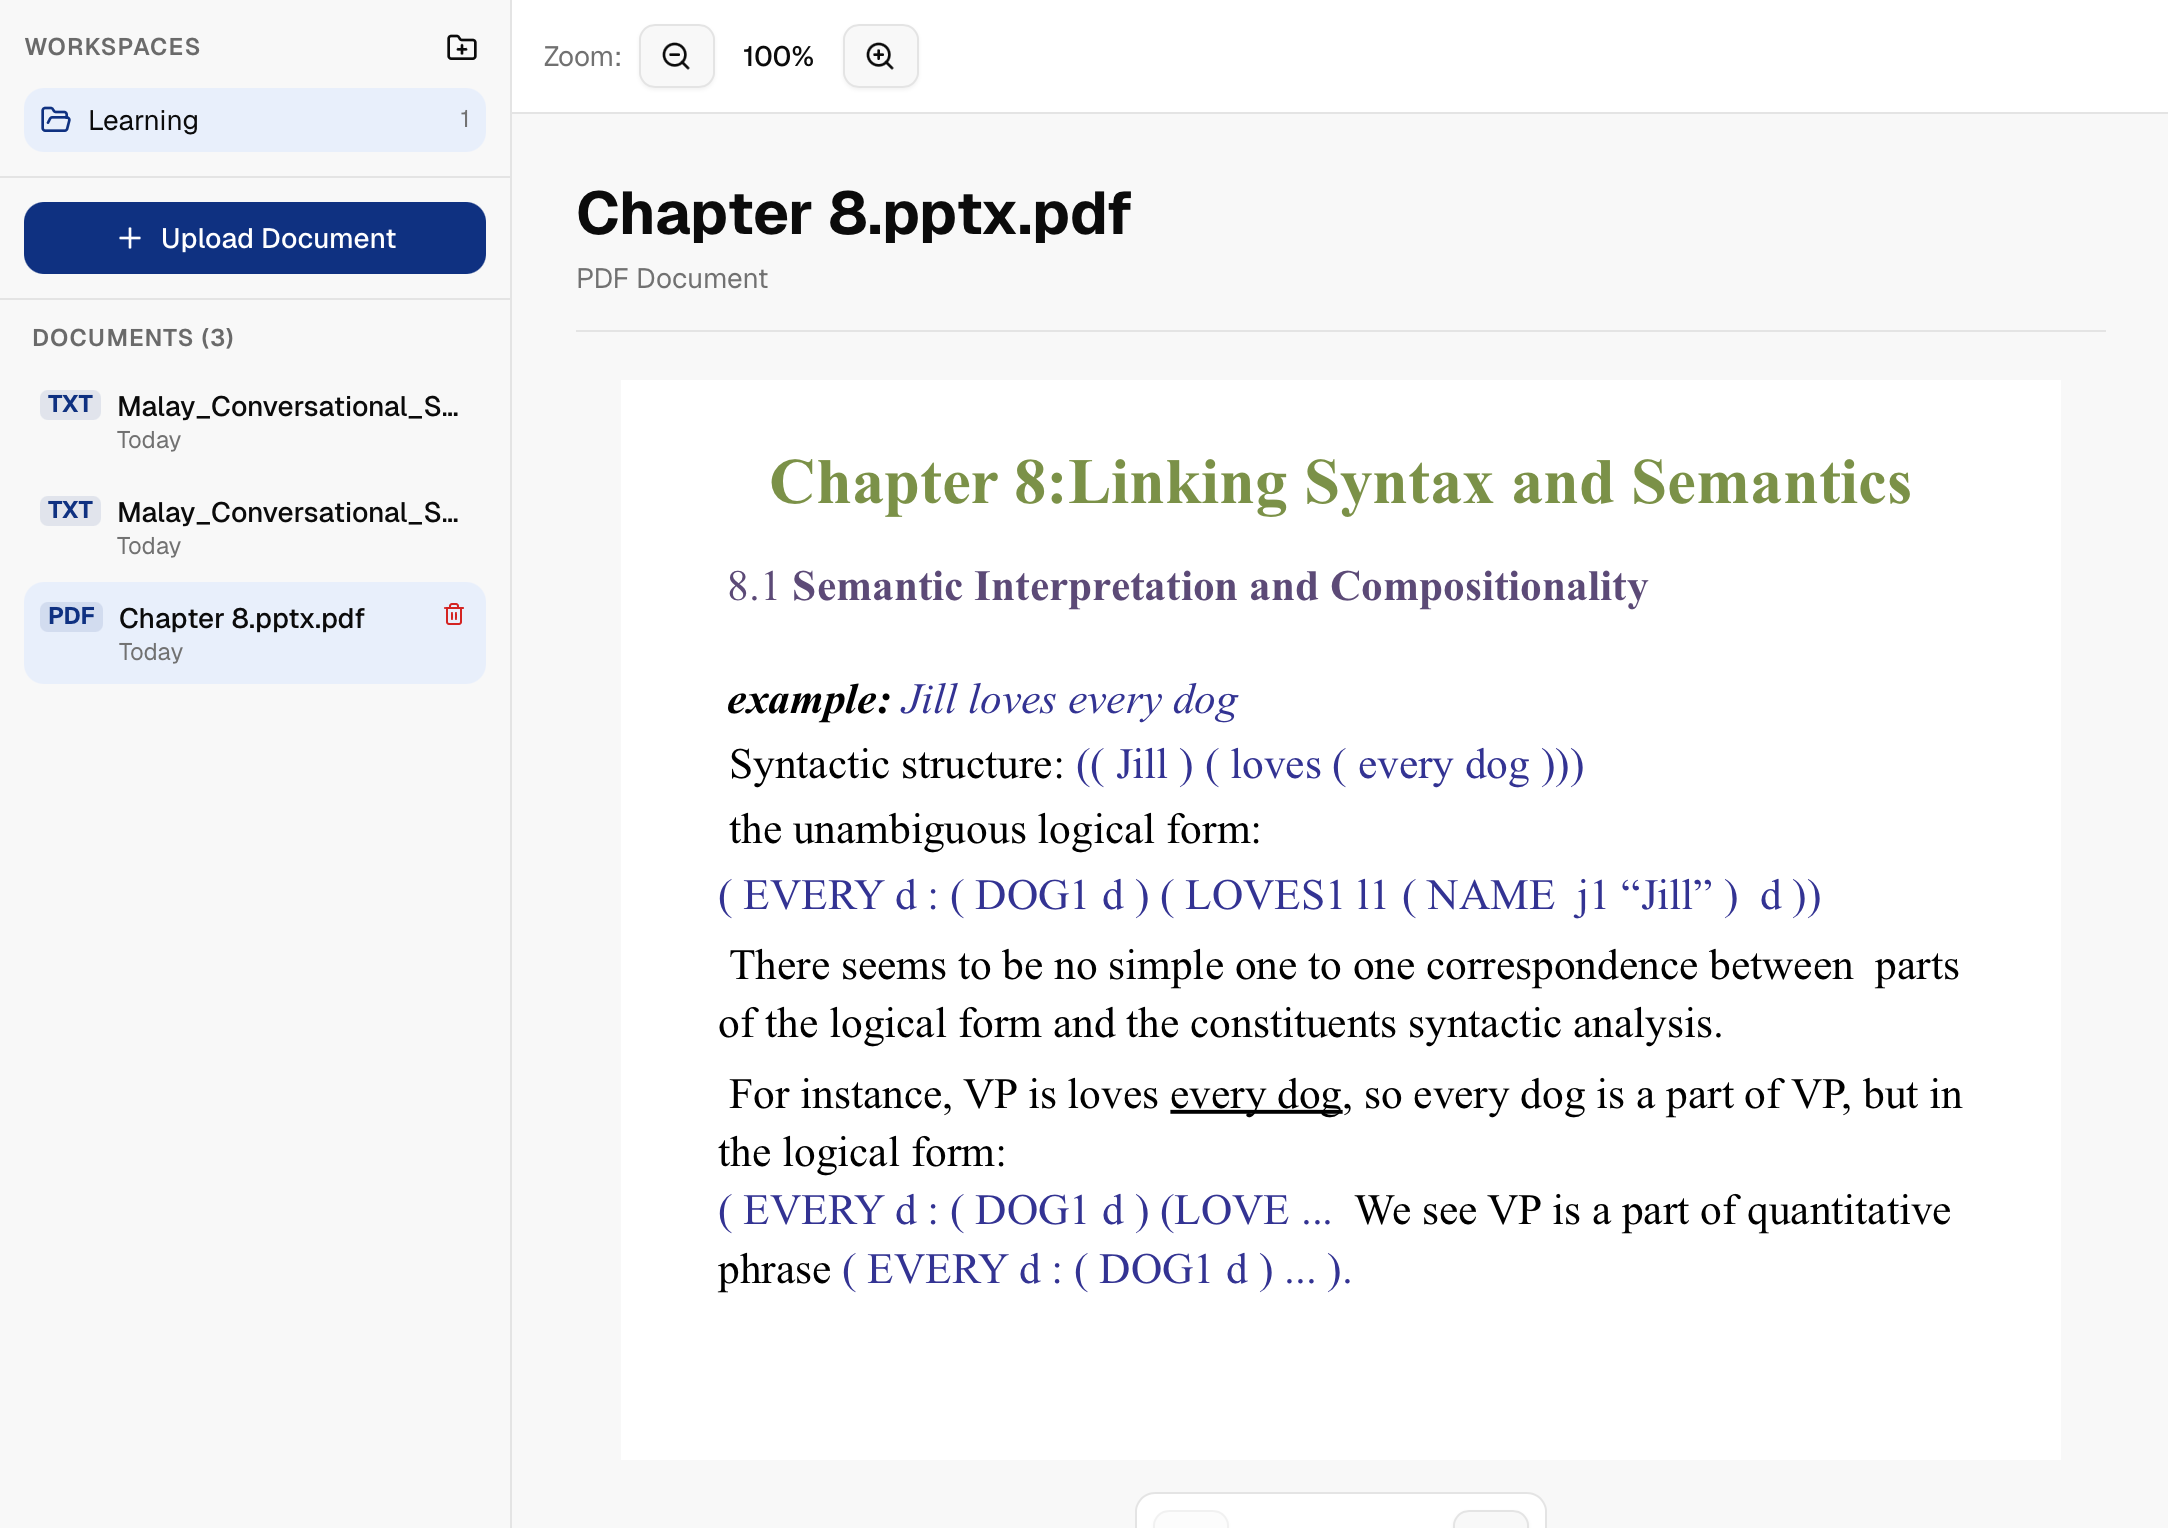
\includegraphics[width=0.88\linewidth]{images/ui-ux/workspace.png}
\end{figure}

\begin{itemize}
    \item \textbf{Nội dung chính.} Hiển thị danh sách tài liệu dưới dạng lưới hoặc danh sách; mỗi thẻ tài liệu bao gồm tên, kích thước, ngày nạp và trạng thái xử lý.
    \item \textbf{Mục tiêu sử dụng.} Giúp người dùng quan sát nhanh toàn bộ thư viện và chọn đúng tài liệu để tiếp tục làm việc.
\end{itemize}

\subsubsection{Không gian làm việc chia đôi}
Đây là giao diện quan trọng nhất, nơi diễn ra tương tác RAG theo thời gian thực.

\begin{figure}[H]
    \centering
    \caption{Giao diện không gian làm việc chia đôi giữa tài liệu và hội thoại}
    \label{fig:ui-split-screen}
    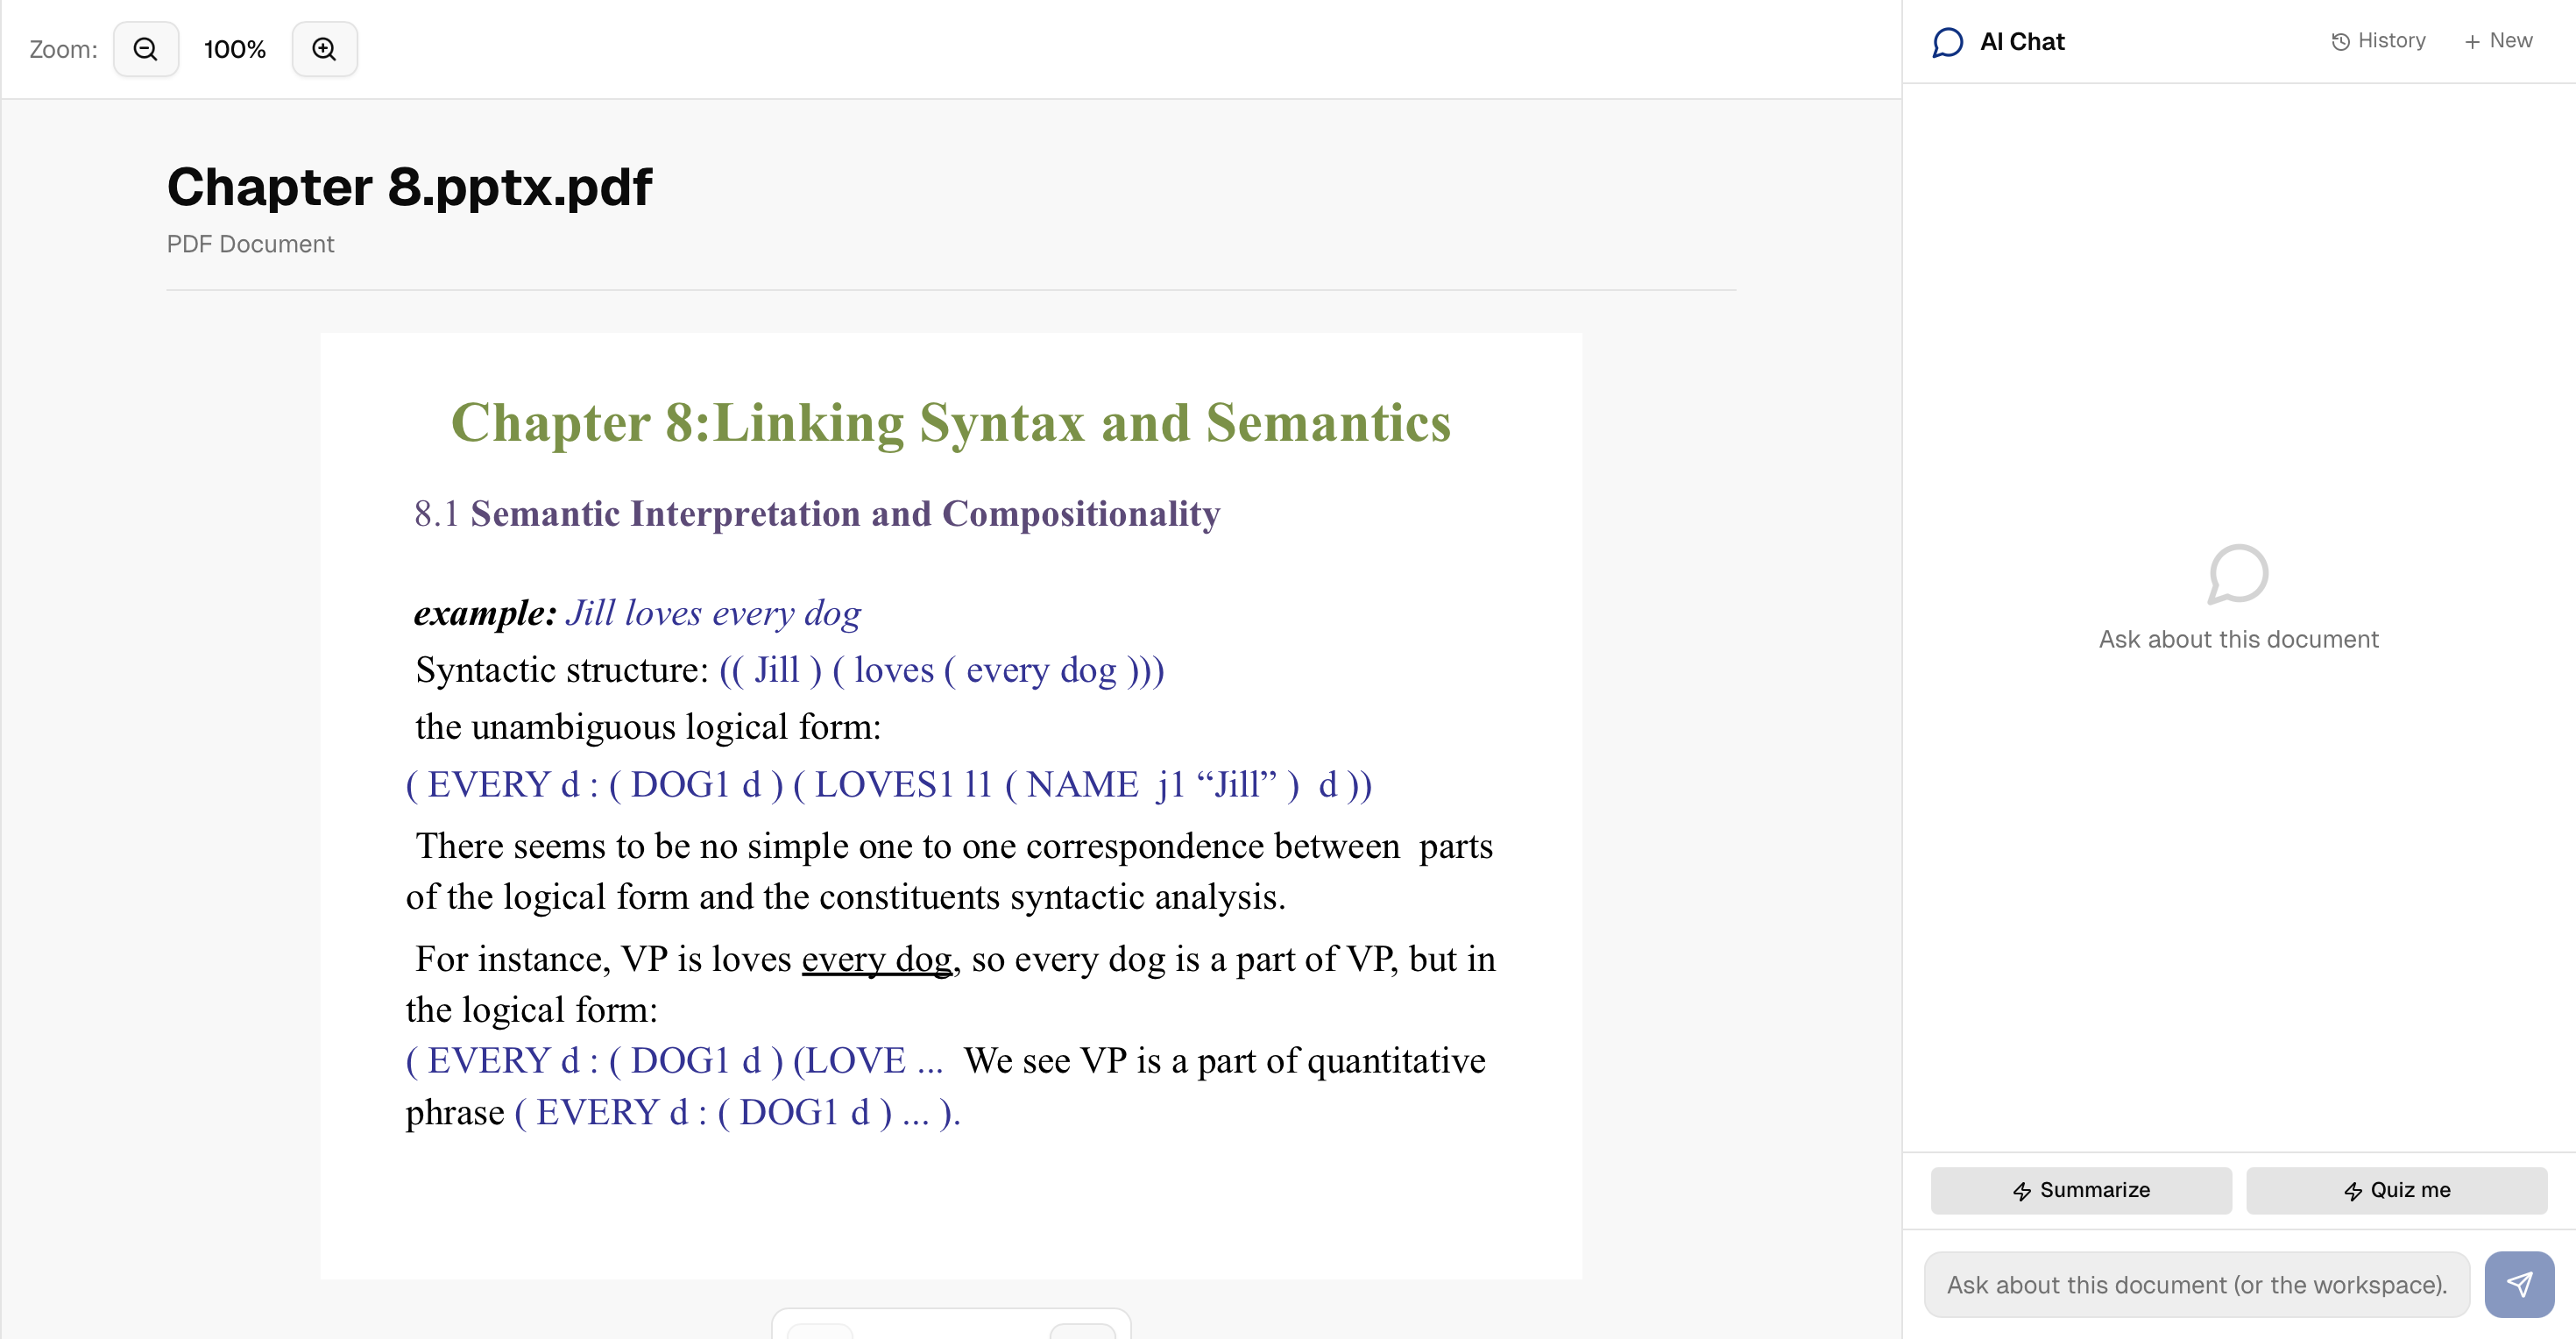
\includegraphics[width=0.92\linewidth]{images/ui-ux/split-screen.png}
\end{figure}

\begin{itemize}
    \item \textbf{Bên trái.} Trình xem tài liệu hiển thị nội dung PDF hoặc văn bản thô với các công cụ như phóng to, thu nhỏ và cuộn độc lập.
    \item \textbf{Bên phải.} Khung chat nơi người dùng đặt câu hỏi và nhận phản hồi kèm trích dẫn.
    \item \textbf{Mục tiêu sử dụng.} Giữ cho người dùng luôn làm việc trong cùng một ngữ cảnh mà không cần chuyển qua lại giữa nhiều cửa sổ.
\end{itemize}

\subsubsection{Cơ chế trích dẫn và liên kết ngược}
Khác biệt quan trọng của UX trong DigitalBookLLM là khả năng kết nối trực tiếp giữa câu trả lời của AI và tài liệu gốc.

\begin{figure}[H]
    \centering
    \caption{Cơ chế trích dẫn và làm nổi bật đoạn văn liên quan trong tài liệu}
    \label{fig:ui-citation}
    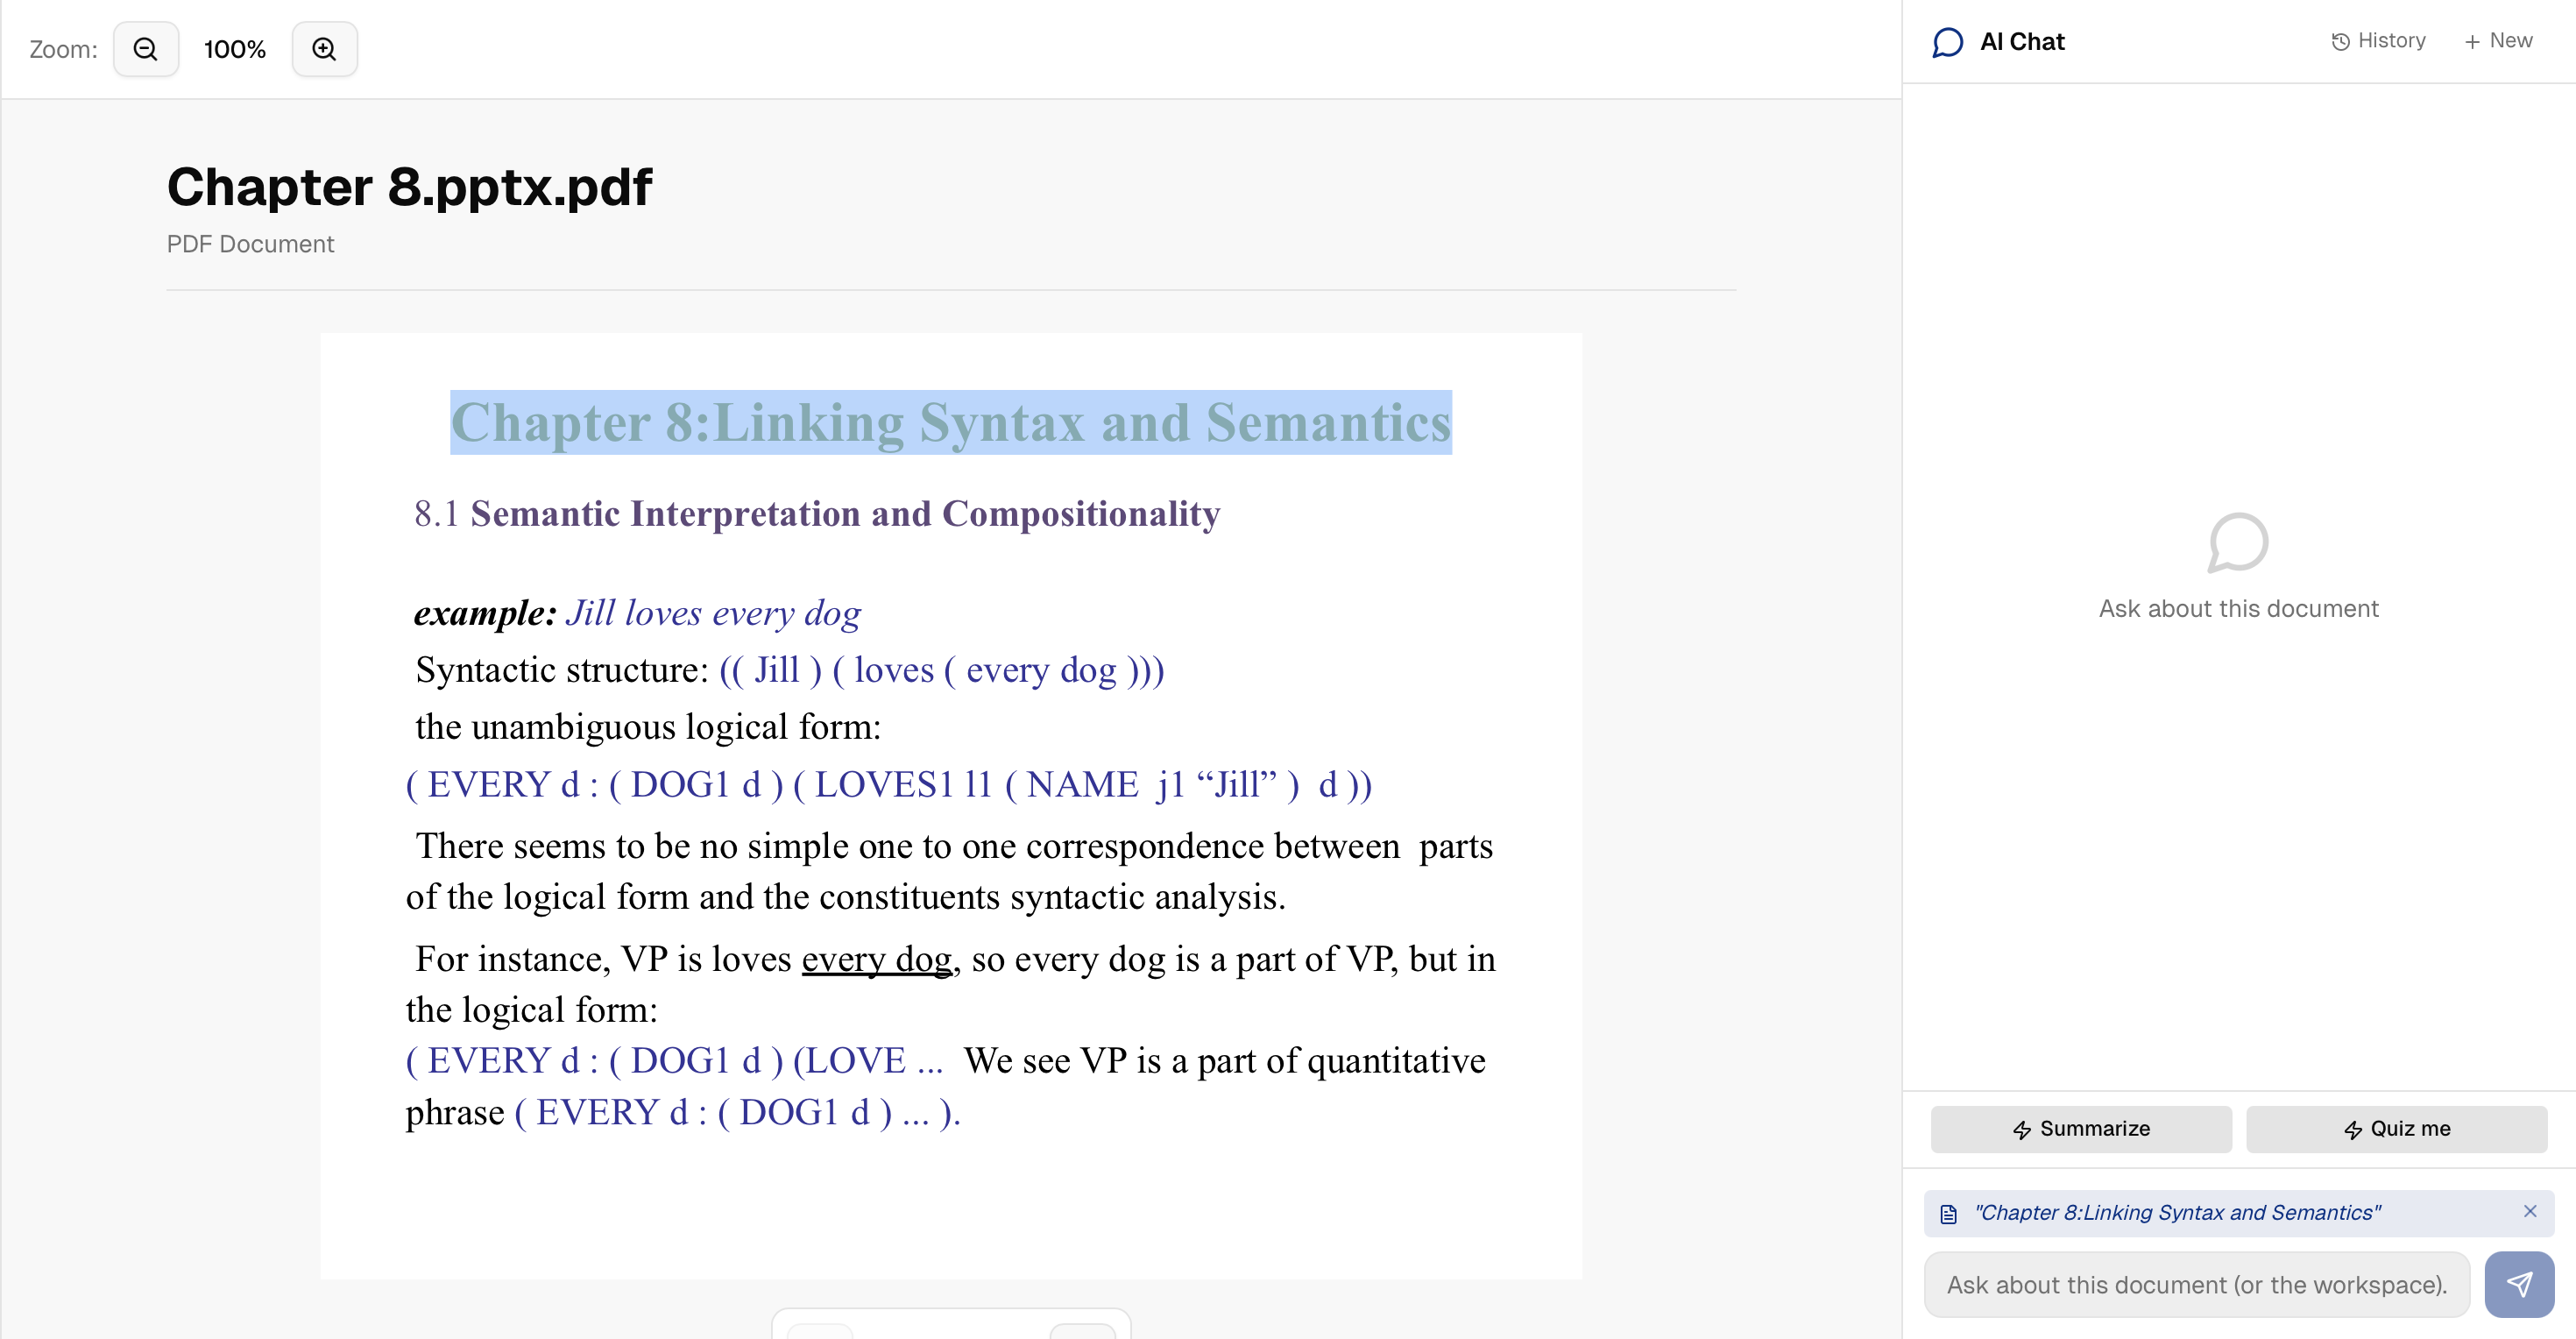
\includegraphics[width=0.92\linewidth]{images/ui-ux/highlight.png}
\end{figure}

\begin{itemize}
    \item \textbf{Cách thức hoạt động.} Các thẻ trích dẫn trong câu trả lời cho phép người dùng nhấp vào và tự động cuộn tài liệu sang vị trí liên quan.
    \item \textbf{Hiệu ứng trực quan.} Đoạn văn bản tương ứng được làm nổi bật để củng cố mối liên hệ giữa phản hồi và nguồn gốc tri thức.
    \item \textbf{Mục tiêu sử dụng.} Tăng độ tin cậy của phản hồi và hỗ trợ quá trình đối chiếu nội dung ngay trên tài liệu nguồn.
\end{itemize}

\subsubsection{Thanh công cụ ngữ cảnh nổi (Contextual Popover)}
Đây là điểm chạm giải quyết trực tiếp bài toán thao tác rườm rà đã nêu ở Chương 1: khi người dùng bôi đen một đoạn văn bản, một thanh công cụ nhỏ hiện ra ngay phía trên vùng chọn với bốn hành động (Highlight, Note, Speak, Ask AI), thay vì buộc người dùng phải mở một menu riêng hay chuyển đổi ứng dụng.

\begin{figure}[H]
    \centering
    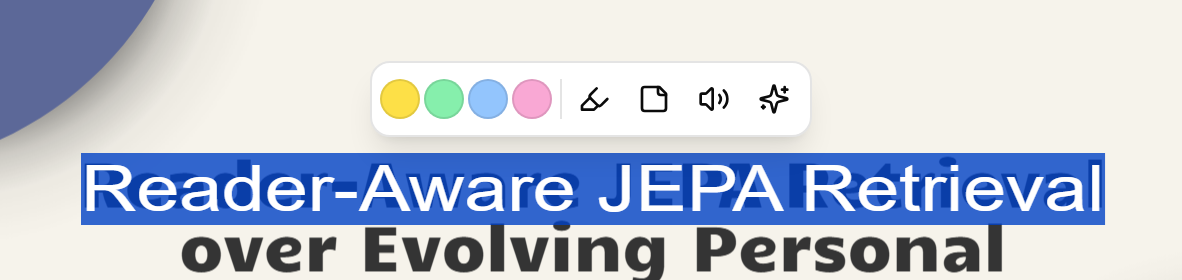
\includegraphics[width=0.92\linewidth]{images/ui-ux/selection-toolbar.png}
    \caption{Thanh công cụ ngữ cảnh hiển thị phía trên vùng văn bản được chọn}
    \label{fig:ui-selection-toolbar}
\end{figure}

\begin{itemize}
    \item \textbf{Highlight.} Mở một bảng chọn màu nhỏ; sau khi chọn, đoạn văn bản được tô màu và lưu lại vị trí (UC-11).
    \item \textbf{Note.} Mở một ô nhập văn bản ngắn để đính kèm ghi chú cá nhân vào đoạn đã chọn.
    \item \textbf{Speak.} Phát âm thanh đọc to đoạn văn bản theo thời gian thực (UC-12).
    \item \textbf{Ask AI.} Focus khung chat, chèn đoạn văn bản đã chọn vào dưới dạng thẻ trích dẫn kèm ba gợi ý câu hỏi nhanh (UC-14).
\end{itemize}

\subsubsection{Màn hình khám phá đồ thị tri thức (Knowledge Graph Explorer)}
Khi chuyển sang Graph Mode, canvas trung tâm hiển thị mạng lưới nút và cạnh biểu diễn các khái niệm người dùng đã tương tác qua nhiều tài liệu và phiên chat (UC-15). Nút được tô màu theo loại thực thể (khái niệm, nhân vật, công nghệ); nhấn vào một nút mở panel chi tiết bên phải, hiển thị mô tả và các đoạn trích dẫn nguồn liên quan.

% \textit{Ảnh chụp màn hình cho mục này chưa có sẵn trong bộ tài nguyên hình ảnh của đồ án; xem tệp theo dõi công việc còn lại để bổ sung.}

\subsection{Khả năng đáp ứng và ngôn ngữ giao diện}
Bố cục chia đôi chuyển thành xếp chồng (trình đọc phía trên, khung chat phía dưới) khi chiều rộng màn hình dưới 768px, với thanh bên (sidebar) thu gọn thành lớp phủ (overlay) trên thiết bị di động. Toàn bộ giao diện hỗ trợ song ngữ Việt/Anh với nút chuyển đổi ở thanh header, đi kèm chế độ sáng/tối/theo hệ thống (UC-09).